%%%%%%%%%%%%%%%%%%%%%%%%%%%%%%%%%%%%%%%%%%%%%%%%%%%%%%%%%%%%%%%%%%%%%%
% LaTeX Example: Project Report
%
% Source: http://www.howtotex.com
%
% Feel free to distribute this example, but please keep the referral
% to howtotex.com
% Date: March 2011
%
%%%%%%%%%%%%%%%%%%%%%%%%%%%%%%%%%%%%%%%%%%%%%%%%%%%%%%%%%%%%%%%%%%%%%%
% How to use writeLaTeX:
%
% You edit the source code here on the left, and the preview on the
% right shows you the result within a few seconds.
%
% Bookmark this page and share the URL with your co-authors. They can
% edit at the same time!
%
% You can upload figures, bibliographies, custom classes and
% styles using the files menu.
%
% If you're new to LaTeX, the wikibook is a great place to start:
% http://en.wikibooks.org/wiki/LaTeX
%
%%%%%%%%%%%%%%%%%%%%%%%%%%%%%%%%%%%%%%%%%%%%%%%%%%%%%%%%%%%%%%%%%%%%%%
% Edit the title below to update the display in My Documents
%\title{Project Report}
%
%%% Preamble
\documentclass[paper=a4, fontsize=11pt]{scrartcl}
\usepackage[utf8]{inputenc}
\usepackage[T1]{fontenc}
\usepackage{fourier}
\usepackage{pgfgantt}
\usepackage{pgfcalendar}
\usepackage[numbers]{natbib}
\bibliographystyle{ieeetr}


\usepackage[english]{babel}															% English language/hyphenation
\usepackage[protrusion=true,expansion=true]{microtype}
\usepackage{amsmath,amsfonts,amsthm} % Math packages
\usepackage[pdftex]{graphicx}
\usepackage{url}

\usepackage{tikz}
\usetikzlibrary{decorations.pathreplacing , chains , intersections}
\usetikzlibrary{calc}
\usepackage{relsize}

%%%% Define custom colors
\definecolor{grisclair}{rgb}{0.7,0.7,0.7}
\definecolor{grisfonce}{rgb}{0.5,0.5,0.5}
\definecolor{green}{RGB}{22,122,48}
\definecolor{red}{RGB}{163,45,29}
\definecolor{blue}{RGB}{20,86,101}
\definecolor{orange}{RGB}{163,96,29}
\definecolor{yellow}{rgb}{0.984375, 0.7265625, 0}


%%% Custom sectioning
%\usepackage{sectsty}
%\allsectionsfont{\centering \normalfont\scshape}


%%% Custom headers/footers (fancyhdr package)
\usepackage{fancyhdr}
\pagestyle{fancyplain}
\fancyhead{}											% No page header
\fancyfoot[L]{}											% Empty
\fancyfoot[C]{}											% Empty
\fancyfoot[R]{\thepage}									% Pagenumbering
\renewcommand{\headrulewidth}{0pt}			% Remove header underlines
\renewcommand{\footrulewidth}{0pt}				% Remove footer underlines
\setlength{\headheight}{13.6pt}


%%% Equation and float numbering
\numberwithin{equation}{section}		% Equationnumbering: section.eq#
\numberwithin{figure}{section}			% Figurenumbering: section.fig#
\numberwithin{table}{section}				% Tablenumbering: section.tab#


%%% Maketitle metadata
\newcommand{\horrule}[1]{\rule{\linewidth}{#1}} 	% Horizontal rule

\title{
		%\vspace{-1in}
		\usefont{OT1}{bch}{b}{n}
		\normalfont \normalsize \textsc{} \\ [25pt]
		\horrule{0.5pt} \\[0.4cm]
		\huge Nouvelles approches de mesure de la rétention dans les files actives VIH \\
		\horrule{2pt} \\[0.5cm]
}
\author{
		\normalfont 								\normalsize
        Grégoire Lurton\\[-3pt]		\normalsize
        %\today
}
\date{}


%%% Begin document
\begin{document}
\maketitle

\section{Contexte et Justification}

Ce projet s'inscrit dans le cadre d'un projet de recherche doctorale sur des méthodes innovantes d'analyse des données de systèmes d'information sanitaire dans les pays à faible ressources. Plus précisément, nous étudions comment adapter la définition des indicateurs et les méthodes de collecte et d'analyse de données pour les adapter à des situations locales ne correspondant pas aux conditions des systèmes statistiques des pays riches.

La mesure de la rétention des patients sous ARV est une mesure clé de la performance des programmes VIH. La chronicité du VIH rend en effet nécessaire une mesure du succès sur le long terme, et la persistence dans le soin des patients est un élément essentiel de cette évaluation. Néanmoins, la mesure de la persistence des patients dans le système de soin est loin d'être triviale, et est largement impactée par les conditions de production des services de soin.

A l'initiation des programmes de traitement du VIH, les professionnels du VIH ont choisi d'utiliser des indicateurs déjà définis et utilisés dans le cadre d'études cliniques, et ont choisi de mesurer la rétention des patients dans le soin par la proportion de patients qui cessent de venir à leurs rendez-vous de suivi\cite{ioannidis_predictors_1999,lebouche_incidence_2006,moh_incidence_2007}.
. La définition de la catégorie Perdu de Vue (PDV) provient donc de programmes pouvant s'appuyer sur des systèmes de collecte de données très performants et mettant en \oe uvre un suivi des patients renforcé. Dans le cadre de programmes de santé publique, cette définition est néanmoins problématique, car elle repose sur une hypothèse de complétude et de qualité des données patients qui est rarement respectée. En définissant les PDV par une absence de données plus que par un élément positif, les différentes définitions des PDV utilisées  mettent en effet dans une même catégorie des patients ayant interrompu leur suivi, et des patients dont les visites n'ont pas été correctement enregistrées. De plus, en basant l'évaluation des programmes sur la catégorisation de certains patients, la mesure d'évaluation a modifié les conditions de soin et les relations entre soignants et soignés \cite{carillon_les_2011}.

De plus, au fur et à mesure que les programmes VIH étaient mis en \oe uvre à travers le monde, il est apparu que cette catégorie était peu spécifique et regroupait des patients dans des situations diverses\cite{kwong-leung_yu_true_2007,dalal_characteristics_2008,mcguire_vital_2010}. Cette faible spécificité pose des problèmes importants pour l'évaluation des programmes de prise en charge du VIH, et plusieurs auteurs ont proposé des méthodes pour corriger la mesure de la rétention. Ces méthodes ont pu se baser sur la collecte de données additionnelles \cite{yiannoutsos_sampling-based_2008,geng_tracking_2010,tassie_evaluation_2010}, ou sur la mise en \oe uvre de modèles de correction \cite{brinkhof_adjusting_2010,egger_correcting_2011,van_cutsem_correcting_2011,henriques_comparison_2012,verguet_incorporating_2013}. Plus récemment, d'autres auteurs ont exploré comment la définition des PDV utilisée par différents programmes peut avoir un impact important sur la mesure de la rétention\cite{chi_empirical_2010,chi_universal_2011,fox_defining_2012,mugavero_measuring_2012,yehia_comparing_2012,grimsrud_impact_2013,shepherd_impact_2013}.

Une hypothèse sous-tendant ces définitions de la rétention est que, si un patient se rend à un rendez-vous, cette visite sera enregistrée correctement dans le système de données correspondant. Il y a donc une équivalence entre la mesure de la rétention et la mesure de la qualité des données dans les centres de santé. Cependant, l'évaluation de cette hypothèse est rarement faite, et son impact sur la mesure du nombre de PDV dans un centre est difficile.

Avec le développement et la mise en \oe uvre croissante de systèmes de dossiers patients informatisés dans les centres de santé, nous disposons d'une opportunité pour améliorer cette situation. La plupart des systèmes informatisés de collecte de données enregistrent en effet des métadonnées sur la saisie des données, comme leur date d'entrée ou le rôle de la personne saisissant les données. Ces métadonnées peuvent être mobilisées pour mesurer la qualité des données, et pour comprendre l'impact de la qualité des données sur la mesure de la rétention.

\section{Objectif de l'étude}

Le projet décrit ici cherche à simuler et à décrire l'impact de la qualité des données collectées dans les centres de santé sur une mesure de la rétention axée sur la catégorie PDV. Cet objectif sera atteint à travers trois objectifs spécifiques :
\begin{description}
	\item[Impact de la qualité des données sur la mesure de la rétention] Nous modéliserons le chemin par lequel la qualité des données affecte la mesure de la rétention, et nous simulerons la mesure des résultats d'une cohorte de prise en charge du VIH en fonction de la qualité de ses données.
	\item[Maturité des données] La capacité des données dans une base de données à mesurer la rétention de patients peut être caractérisée par le temps s'écoulant entre un évènement et l'enregistrement de cet évènement. Nous définirons une mesure de \textit{maturité des données}, pour décrire la capacité d'une base de données à mesurer la rétention dans une cohorte. Cette mesure sera testée et validée sur la cohorte simulée.
	\item[Mesures robustes de la rétention] A partir des connaissances obtenues avec les objectifs précédents, nous définirons, testerons et validerons des mesures de la rétention dans les cohortes VIH qui seront robustes à la qualité des données. Ces mesures seront évaluées sur la capacité à bien mesurer la rétention des patients sur notre cohorte simulée, et sur leur robustesse aux variations de qualité des donnée.
\end{description}

\section{Méthode}
\subsection{Cadre théorique}
\label{sec:theory}

\subsubsection{Processus de suivi du VIH}

Les patients VIH se rendent à des rendez-vous réguliers dans leur centre de traitement. A chaque visite, un rendez-vous est fixé pour leur prochaine visite. La date de la $v$\^{ème} visite du patient $i$ est notée $V_v^i$, et la date du rendez-vous qui était fixé pour cette visite est notée $A_v^i$. Si $V_v^i < A_v^i$, le patient est venu en avance à son rendez-vous. Si $V_v^i > A_v^i$, le patient est venu en retard. On note $l_v^i = A_v^i - V_v^i$, le temps écoulé entre le rendez-vous fixé et la visite effective. La Figure \ref{fig:late_days} montre la distribution de $l_v^i$ dans nos données.


\begin{center}
\begin{figure}[h]
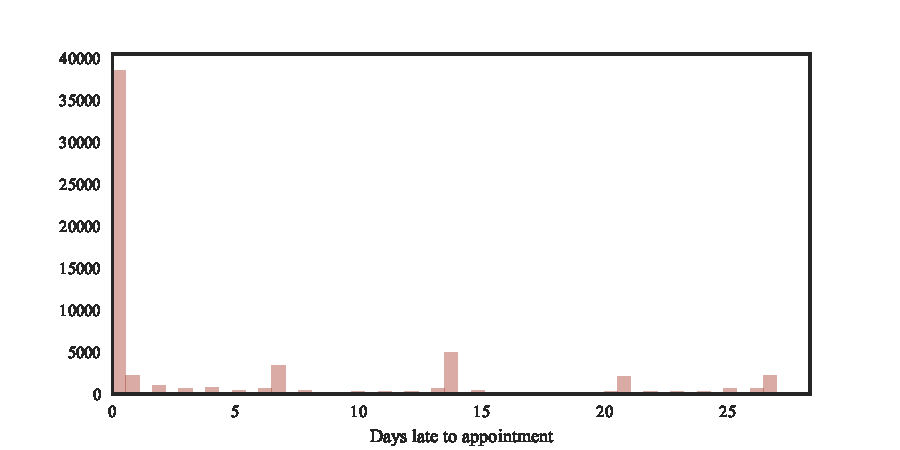
\includegraphics[width=\textwidth]{figure/time_late_to_appointment.pdf}
\caption{Distribution de $l_v^i$ dans nos données.}
\label{fig:late_days}
\end{figure}
\end{center}

Le délai entre une visite et la date de prochain rendez-vous donné est défini par les normes et directives nationales sur le suivi des patients sous ARV. Les patients suivis depuis plus longtemps auront en moyenne des temps entre visites plus longs que les patients enrôlés plus récemment. On note $\bar{f}_v^i$ la fréquence de visite du patient $i$ à la visite $v$. Cette unité est souvent un multiple de 28 jours, du fait que les patients ont souvent des jours privilégiés pour planifier leurs visites médicales. La Figure \ref{fig:schedule_days} montre la distribution de $\bar{f}_v^i$ dans nos données.

\begin{center}
\begin{figure}[h]
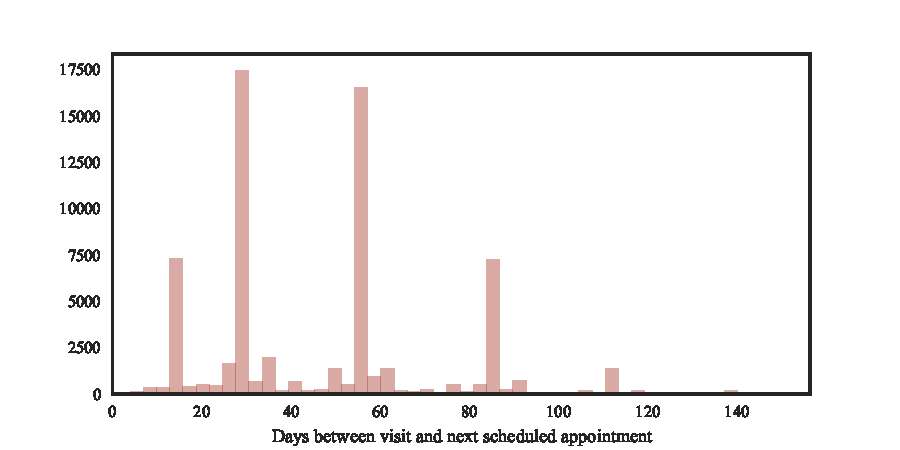
\includegraphics[width=\textwidth]{figure/time_to_appointment.pdf}
\caption{Distribution of $\bar{f}_v^i$ in our data.}
\label{fig:schedule_days}
\end{figure}
\end{center}

Finalement, le temps entre deux visites peut être décrit comme :
$$V_{v+1}^i - V_v^i = \bar{f}_v^i + l_v^i  $$

\subsubsection{Processus d'entrée des données}

La date à laquelle une visite est enregistrée dans une base de dossiers informatisées est notée $R(V_v^i)$. Par définition, $R(V_v^i) \geq V_v^i$, et le délai pour l'enregistrement des données est noté:
$$R(V_v^i) - V_v^i = \delta_v^i \ geq 0$$

Dans certains cas, une visite ne sera jamais enregistrée, nous noterons cette situation $\delta_v^i \rightarrow \infty$. $\delta_v^i$ peut varier dans un centre de santé, en fonction de la charge de travail, des ressources humaines ou d'autres facteurs. La Figure \ref{fig:data_entry_time} montre la distribution de $\delta_v^i$ dans nos données.

\begin{center}
\begin{figure}[h]
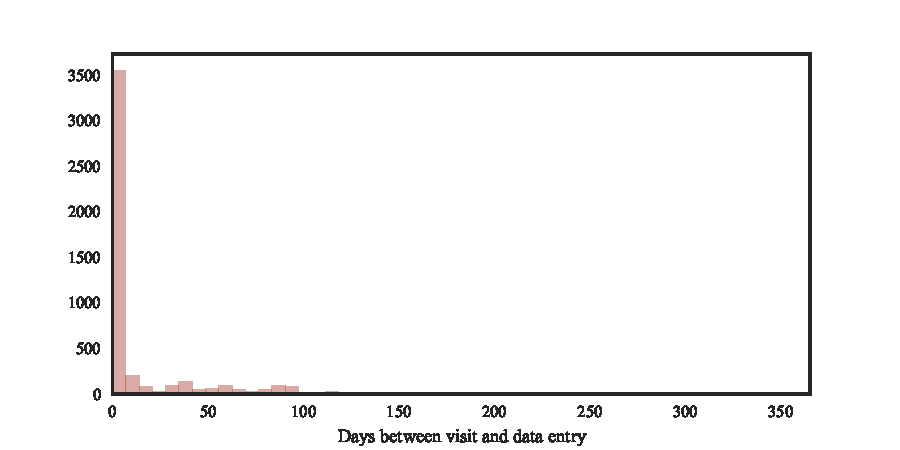
\includegraphics[width=\textwidth]{figure/data_entry_time.pdf}
\caption{Distribution of $\delta_v^i$ in our data.}
\label{fig:data_entry_time}
\end{figure}
\end{center}

Finalement, l'enregistrement des données est clos à la date $T_{close}$ avant que les données ne soient analysées. Pour simplifier, la date de cloture de la base de données sera assimilée à la date d'analyse, quitte à relaxer cette hypothèse lors de notre travail sur la maturité des données.


\pgfdeclarelayer{background}
\pgfdeclarelayer{foreground}
\pgfsetlayers{background,main,foreground}
\begin{center}
 \begin {figure}[h]
        \centering
\resizebox{\linewidth} {!} {
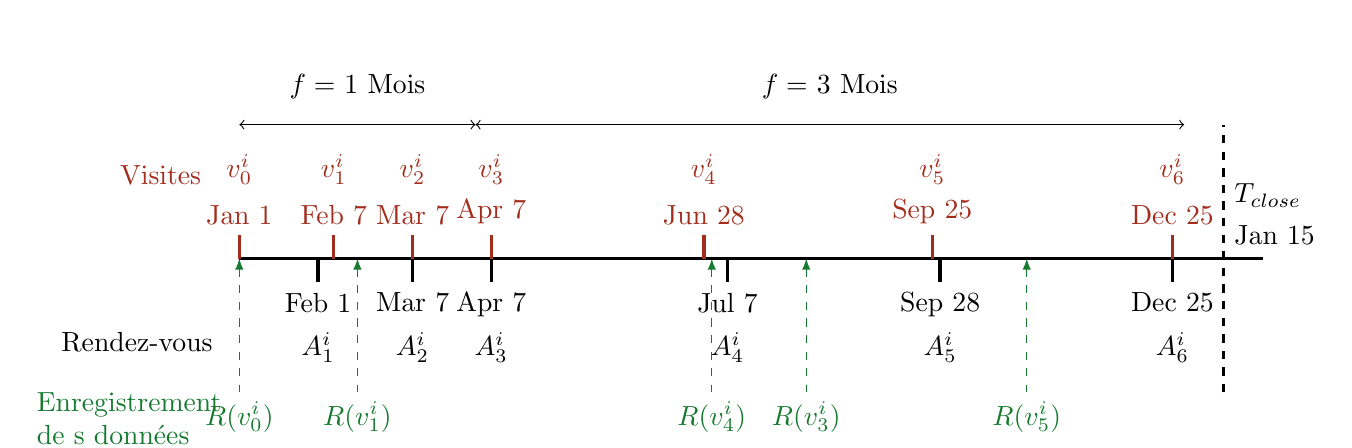
\begin{tikzpicture}


  \draw[<->] (0,1.7) -- (3,1.7);
  \draw[] (1.5,1.9) node[above]{$f =$ 1 Mois};
  \draw[<->] (3,1.7) -- (12,1.7);
  \draw[] (7.5,1.9) node[above]{$f =$ 3 Mois};


  \draw[ very thick] (0,0) -- (13,0);

\begin{pgfonlayer}{main}
  %% Draw Appointments
  \draw[very thick] (-1.3,-8mm)node[below]{Rendez-vous};
  \foreach \x/\y/\z in {1/Feb 1/$A_1^i$,
                     2.2/Mar 7/$A_2^i$,
                     3.2/Apr 7/$A_3^i$,
                     6.2/Jul 7/$A_4^i$,
                     8.9/Sep 28/$A_5^i$,
                     11.85/Dec 25/$A_6^i$
                     }{
 \draw[very thick] (\x, 0) --+ (0,-3mm) node[below](\x){\fontsize{20}{22.4}\y}(\x,-8mm)node[below]{\z};
 }


  %% Draw Visits
  \draw[red , very thick] (-1,8mm)node[above]{Visites};
  \foreach \x/\y/\z in {0/Jan 1/$v_0^i$ ,
                     	1.2/Feb 7/$v_1^i$,
                     	2.2/Mar 7/$v_2^i$,
                     	3.2/Apr 7/$v_3^i$,
                     	5.9/Jun 28/$v_4^i$,
                     	8.8/Sep 25/$v_5^i$,
						11.85/Dec 25/$v_6^i$
                        }{
	\draw[red , very thick] (\x, 0) --+ (0,3mm) node[above](\x){\fontsize{20}{22.4}\y}(\x,8mm)node[above]{\z};
    }
\end{pgfonlayer}

	%\fontsize{20}{22.4}

\begin{pgfonlayer}{background}
    %% Draw Data Entry
    \draw[very thick ,  green] (-1.4,-25mm)node[above , align=left]{Enregistrement\\de s données};
    \foreach \x/\y in {0/$R(v_0^i)$,
  					   1.5/$R(v_1^i)$,
					   6/$R(v_4^i)$,
                       7.2/$R(v_3^i)$,
                       10/$R(v_5^i)$
                        }{
    \draw[dashed ,  green , latex-] (\x,0mm) -- +(0,-17mm)node[below]{\y};
    }

\draw[dashed ,  very thick] (12.5,-17mm) -- (12.5,17mm) ;
\draw[very thick] (12.5, 8mm)node[right]{$T_{close}$};
\draw[very thick] (12.5, 3mm)node[right]{Jan 15};

\end{pgfonlayer}

\end{tikzpicture}
}
\caption{Individual follow-up and data entry process}
\label{fig:timeline-followup}
\end{figure}
\end{center}

La Figure \ref{fig:timeline-followup} montre comment les différents paramètres que nous venons de définir s'agencent pour un suivi de patient donné. Ce patient imaginaire a eu une première visite le 1$^{er}$ janvier, et a eu un rendez-vous fixé pour le 1$^{er}$ février. Il est venu à ce rendez-vous avec 6 jours de retard. Après trois mois de suivi mensuel, il est passé à un suivi trimestriel. Il est venur en avance à son rendez-vous du mois de juillet, et est venu à tous ses rendez-vous jusqu'à la fin de l'année. Les données ont été enregistrées très rapidement en début d'année, mais $V_2^i$ n'a jamais été enregistrée. $V_4^i$ a été enregistrée avant $V_3^i$, et $V_6^i$ n'a pas pu être enregistrée avant la cloture de la base de données pour analyse, le 15 janvier de l'année suivante. Cet exemple donne une démonstration rapide des différentes situations qui peuvent être rencontrées lors de l'analyse de données de suivi patient.

\subsubsection{Définition des Perdus de Vue}

Une pièce centrale de la définition des PDV est la \textit{période de grace} au cours de laquelle un patient, même si il a manqué un rendez-vous fixé, est toujours considéré suivi. Cette \textit{période de grace} est notée $G_0$.

Un patient $i$ est considéré activement suivi si il n'est pas en retard à son dernier rendez-vous $v^*$ de plus de  $G_0$  jours.

$$l_v^{*}^i \leq  G_0$$

En considérant cette situation, on voit qu'elle regroupe trois situations différentes :
\begin{enumerate}
\item Le patient est PDV et ne reviendra jamais dans le centre de santé
\item Le patient est en retard à son rendez-vous mais reviendra plus tard et $l_v^{*}^i > G_0$
\item Le patient est venu pour son rendez-vous $v^{*} + 1$ mais $\delta_{v^*+1}^i > G_0$.
\end{enumerate}

En utilisant cette définition, on peu exprimer la probabilité qu'une patient soit identifié comme PDV à partir des données disponibles. On défini  $X = 1$ le fait qu'un patient soit activement suivi, et  $X = 0$ un patient PDV. On a donc $p(X = 0 | l_v^{*}^i \leq  G_0)$

$$p(X = 0 | l_v^{*}^i \leq  G_0) = 1 - p(X = 1  \cap l_v^{*}^i \leq  G_0) - p(\delta_{v^*+1}^i > G_0) $$

Using this definition, we can express the probability that a LTFU patient is identified based on the data at hand. Indeed, definin gthe event that a patient is actively in care, and $X = 0$ if the patient is LTFU. We can thus get $p(X = 0 | l_v^{*}^i \leq  G_0)$ as the combination of elements we can measure :

$$p(X = 0 | l_v^{*}^i \leq  G_0) = 1 - p(X = 1  \cap l_v^{*}^i \leq  G_0) - p(\delta_{v^*+1}^i > G_0) $$

On voit que $X = 1  \cap l_v^{*}^i \leq  G_0$ peut être vu comme l'expression de la qualité des données, et $\delta_{v^*+1}^i > G_0$ est la myopie intrinsèque du système d'information. Parvenir à faire la différence entre ces deux termes est essentiels pour comprendre la rétention des patients dans la file active et son incertitude.

\section{Données}

Dans l'état actuel du projet, nous disposons de données issues d'une base de dossiers patients informatisés obtenus auprès du programme VIH du Kenya dans le cadre de l'étude ABCE à l'Institute for Health Metrics and Evaluation (IHME). Dans ce centre de santé, 4833 patients ont été enregistrés pour leur suivi VIH, de 2005 à juin 2012, et 69591 visites ont été enregistrées sur cette période. Le délai d'entrée des données est disponible pour au moins 4853 de ces visites.

Nous souhaitons ajouter d'autres bases de données de dossiers patients informatisés à notre étude pour varier à la fois les délais de rendez-vous, et les conditions d'entrée des données. En Haïti, les données du système ISanté présentent sont à la fois une opportunité en terme de nombre de patients suivis, et de durée de suivi, qui nous permettent de bien évaluer la variance de nos différents paramètres par sites et dans le temps.

Ces données sont analysées anonymement et en agrégat. Pour chaque patient, nous n'utilisons que les dates de visites planifiées et effectives. En cas d'absence des dates de rendez-vous, nous imputons des dates de rendez-vous en fonction des pratiques apparentes dans les données. Nous utilisons aussi les métadonnées enregistrées par les systèmes de collecte de données. En particulier, comme expliqué plus haut, nous utilisons les dates d'enregistrement des données pour produire une mesure de la qualité des données disponibles.

Nous ne rapportons pas de données précises sur les résultats du programme de prise en charge, et toutes les données disponibles sont utilisées pour informer les paramètres de simulation de la cohorte VIH.

\section{Méthodes}

Notre travail sera effectué en trois étapes principales. Dans un premier temps, nous estimerons les paramètres nécessaires à notre modèle, à partir des données disponibles. Dans un second temps, nous simulerons une cohorte ainsi que le processus de collecte de données correspondant. Finalement, nous utiliserons ces simulations pour répondre les questions qui nous intéressent.

\paragraph{Modélisation -} Les différents paramètres présentés dans la section \ref{sec:theory} seront estimés à partir des cohortes pour lesquelles nous disposerons de dossiers informatisés. Nous utiliserons une approche bayésienne, et estimerons les distributions postérieures de nos paramètres d'intérêt sur lesquelles nous simulerons les réalisations des paramètres à inclure dans la simulation.

\paragraph{Simulation -} A partir des paramètres estimés à l'étape précédente, nous simulerons une cohorte de suivi de patient VIH sur plusieurs années. Cette simulation sera faite en utilisant le cadre du Cost Effectiveness Analysis Microsimulation (CEAM), développé à IHME pour simuler des files actives.

Dans un second temps, nous simulerons le processus d'enregistrement des données, pour chaque mois, en simulant un  $\delta$ pour chaque visite ayant été simulée à l'étape précédente. Nous obtiendrons ainsi une date de saisie pour chacune de ces visites. Nous disposerons donc finalement de toute l'information nécessaire pour estimer la rétention et mesurer la rétention d'une cohorte donnée. En renouvelant l'exercice en variant les paramètres, nous pourrons estimer les paramètres d'intérêt pour les objectifs de notre étude.

\paragraph{Paramètre d'intérêt - }A partir de ces données simulées, nous serons donc en mesure de mesurer les éléments suivants.
\begin{enumerate}
\item{Impact de la qualité des données} Nous simulerons et mesurerons $ p(X = 0 | \theta_{\delta})$ avec différentes valeurs du paramètre $\theta_{\delta}$. Plusieurs scénarios différents seront estimés pour la qualité des données, en variant à la fois la moyenne et la variance de $\delta$. Une qualité de donnée parfaite sera comparée à des situations avec des longs délais de saisie de données, et des situations avec d'importantes pertes de données (grande variance de $l$). Les variations de $p$  qui seront alors observées seront décrites comme l'impact de la qualité des données sur la mesure de la rétention.

\item{Maturité des données} Au fur et à mesure que les données sont saisies, ou que des patients ayant manqué des visites réintègrent leur suivi, les données d'une certaine période sont complétées. Au fur et à mesure que la maturité des données augmente, la variance due à la qualité des données diminue. Faire varier $T_close$, peut donc avoir un impact sur la mesure de la rétention d'un patient à une date donnée. Nous mesurerons la rétention de notre cohorte simulée en utilisant plusieurs dates de cloture de la base de données. Ces mesures nous permettrons de définir et tester une mesure de la maturité des données, à partir d'une combinaison de  $\bar{f}$, $l$ et $\delta$ qui nous permettra d'identifier une date minimale optimale d'analyse pour estimer la rétention dans un programme, et une période de grace optimale $G_0$ à utiliser pour différents niveaux de maturité.

\item{Mesures robustes de la rétention} Finalement, nous explorerons des mesures de la rétention plus robustes que le taux de PDV utilisé. Ces mesures pourront inclure:
\begin{itemize}
	\item Le ratio du nombre mensuel moyen de visites, corrigé pour la qualité des données, divisé par le nombre de visites attendues.
	\item Le ratio du nombre de nouveau au nombre d'anciens patients.
	\item La probabilité que le taux de PDV est plus haut qu'un palier standard fixé.
\end{itemize}
\end{enumerate}

Pour chacune de ces mesures, nous évaluerons leur capacité à mesurer la rétention dans la file active, en les comparant à la méthode de référence avec données parfaites. Nous évaluerons aussi la sensibilité de ces mesures à la qualité et à la maturité des données.

\section{Agenda Prévisionnel}

\begin{figure}[!t]
	\begin{ganttchart}[vgrid,hgrid,
	y unit chart=.6cm]{1}{18}
		\gantttitle{2017}{12}
		\gantttitle{2018}{6} \\
		\gantttitlelist{1,...,12}{1} \gantttitlelist{1,...,6}{1}\\

		\ganttset{bar/.append style={draw=red!40 , fill=red!40},
					group/.append style={draw=red, fill=red}}
		\ganttbar{Data Extraction}{1}{4} \\
		\ganttbar{Modeling and Model estimation}{5}{6} \\
		\ganttbar{Cohort Simulation}{7}{9} \\
		\ganttmilestone{Sharing Cohort simulation results}{9} \\
		\ganttbar{Data Quality Impact}{10}{10} \\
		\ganttbar{Data Maturity}{11}{12} \\
		\ganttbar{Robust Measures of retention}{13}{14} \\
		\ganttmilestone{Sharing Final Results}{14} \\
		\ganttbar{Paper Writing}{15}{16} \\
		\ganttmilestone{Paper Submission}{16}
	\end{ganttchart}
	\caption{Gantt Chart for Aim 1}
	\label{GanttPaper1}
\end{figure}


\section{Références}
\bibliography{bibliographie}

\end{document}
